\chapter{Metodologi Penelitian}
Pada bab ini, dijelaskan tentang tahapan-tahapan penelitian yang dilakukan untuk menyelesaikan masalah yang telah dikemukakan pada rumusan masalah. Ditunjukkan pula jadwal penelitian untuk masing-masing tahapan penelitian tersebut.
\section{Metode Penelitian}
Metode penelitian dapat dilihat pada Gambar~\ref{fig:metodologi_penelitian}.

\begin{figure}[H]
    \centering
    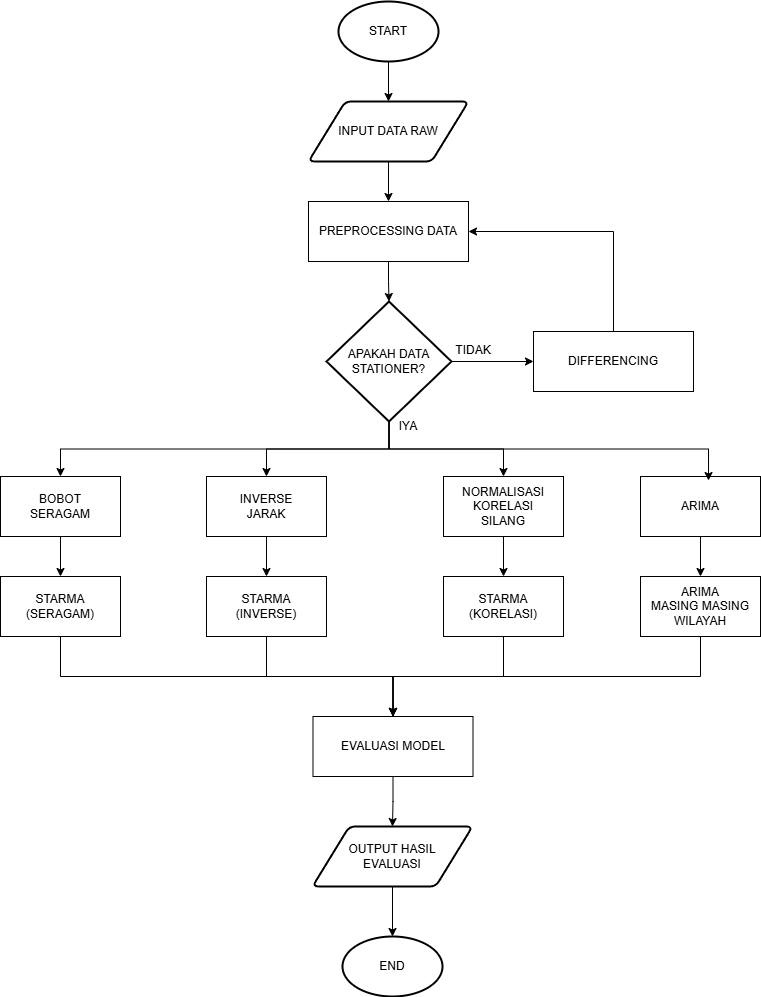
\includegraphics[width=0.6\textwidth]
    {images/bab_3/flowchart}
    \caption{Diagram Alur Metodologi Penelitian}
    \label{fig:metodologi_penelitian}
\end{figure}
\section{Sumber Data}
Penelitian ini dilakukan menggunakan data sekunder secara daring tanpa melakukan pengambilan data di lapangan. Seluruh proses analisis dan pengolahan data dilakuakn secara komputasi di lingkugan pengolahan data statistik. Penelitian ini berlangsung dalam rentang waktu Januari hingga Juni 2025. 

Data utama yang digunakan dalam penelitian ini adalah data curah hujan harian berbasis satelit yang diperoleh dari NASA \textit{(National Aeronnautics and Space Administration)} melalui platform \textit{ POWER Data Access Viewer}. Data ini mencakup informasi spasial (koordinat grid wilayah) dan temporal (periode waktu pengamatan) yang diperlukan dalam pemodelan spasio temporal menggunakan STARMA. 

Selain itu, informasi koordinat geografis yang merepresentasikan lokasi grid atau titik observasi juga digunakan untuk membangun \textit{spatial weight matrix} yang merepresentasikam kedekatakan spasial antar wilayah. Data pendukung ini diambil langusng dari metadata bawaan dataset NASA yang digunakan. 
Berikut merupakan gambar sumber data yang digunakan dalam penelitian ini:
\begin{figure}[H]
    \centering
    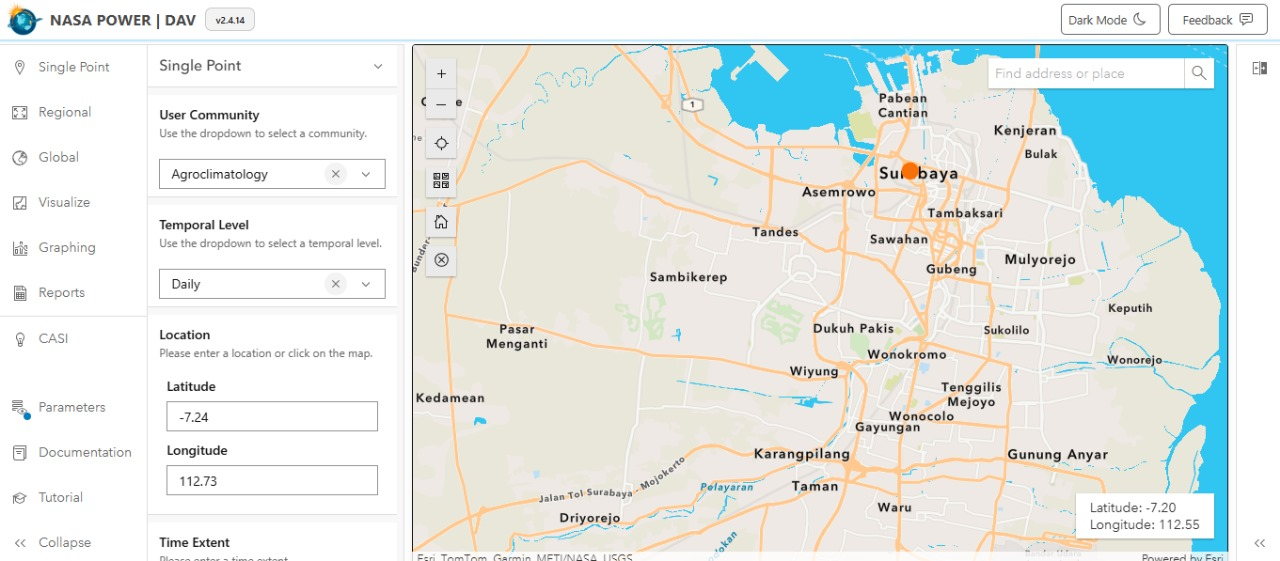
\includegraphics[width=0.9\textwidth]{images/bab_3/nasa.jpg}
    \caption{Data NASA Wilayah Surabaya}
    \label{fig:flowchart-pemodelan}
\end{figure}

\subsection{Data Sekunder}
\begin{longtable}{|l|c|c|c|c|}
    \caption{Data Curah Hujan Bulanan Berdasarkan Wilayah}
    \label{table:data_sekunder} \\
    \hline
    \textbf{Wilayah} & \textbf{Latitude} & \textbf{Longitude} & \textbf{Date} & \textbf{Precipitation} \\
    \hline
    \endfirsthead

    \hline
    \textbf{Wilayah} & \textbf{Latitude} & \textbf{Longitude} & \textbf{Date} & \textbf{Precipitation} \\
    \hline
    \endhead

    \hline
    \endfoot

    \hline
    \endlastfoot

    % ================= UTARA =================
    Utara  & -7.2 & 112.73 & 1/31/2015 & 13.89 \\
    Utara  & -7.2 & 112.73 & 2/28/2015 & 11.93 \\
    Utara  & -7.2 & 112.73 & 3/31/2015 & 9.38 \\
    \multicolumn{1}{|c|}{\raisebox{0.5ex}{$\vdots$}} &
    \multicolumn{1}{c|}{\raisebox{0.5ex}{$\vdots$}} &
    \multicolumn{1}{c|}{\raisebox{0.5ex}{$\vdots$}} &
    \multicolumn{1}{c|}{\raisebox{0.5ex}{$\vdots$}} &
    \multicolumn{1}{c|}{\raisebox{0.5ex}{$\vdots$}} \\  
    Utara  & -7.2 & 112.73 & 10/31/2024 & 1.12 \\
    Utara  & -7.2 & 112.73 & 11/30/2024 & 6.53 \\
    Utara  & -7.2 & 112.73 & 12/31/2024 & 13.60 \\
    \hline

    % ================= BARAT =================
    Barat  & -7.24 & 112.61 & 1/31/2015 & 13.92 \\
    Barat  & -7.24 & 112.61 & 2/28/2015 & 11.87 \\
    Barat  & -7.24 & 112.61 & 3/31/2015 & 9.44 \\
    \multicolumn{1}{|c|}{\raisebox{0.5ex}{$\vdots$}} &
    \multicolumn{1}{c|}{\raisebox{0.5ex}{$\vdots$}} &
    \multicolumn{1}{c|}{\raisebox{0.5ex}{$\vdots$}} &
    \multicolumn{1}{c|}{\raisebox{0.5ex}{$\vdots$}} &
    \multicolumn{1}{c|}{\raisebox{0.5ex}{$\vdots$}} \\  
    Barat  & -7.24 & 112.61 & 10/31/2024 & 1.46 \\
    Barat  & -7.24 & 112.61 & 11/30/2024 & 6.29 \\
    Barat  & -7.24 & 112.61 & 12/31/2024 & 13.62 \\
    \hline

    % ================= TIMUR =================
    Timur  & -7.31 & 112.84 & 1/31/2015 & 12.24 \\
    Timur  & -7.31 & 112.84 & 2/28/2015 & 10.29 \\
    Timur  & -7.31 & 112.84 & 3/31/2015 & 8.84 \\
    \multicolumn{1}{|c|}{\raisebox{0.5ex}{$\vdots$}} &
    \multicolumn{1}{c|}{\raisebox{0.5ex}{$\vdots$}} &
    \multicolumn{1}{c|}{\raisebox{0.5ex}{$\vdots$}} &
    \multicolumn{1}{c|}{\raisebox{0.5ex}{$\vdots$}} &
    \multicolumn{1}{c|}{\raisebox{0.5ex}{$\vdots$}} \\  
    Timur  & -7.31 & 112.84 & 10/31/2024 & 1.22 \\
    Timur  & -7.31 & 112.84 & 11/30/2024 & 5.63 \\
    Timur  & -7.31 & 112.84 & 12/31/2024 & 12.31 \\
    \hline

    % ================= SELATAN =================
    Selatan & -7.35 & 112.73 & 1/31/2015 & 14.30 \\
    Selatan & -7.35 & 112.73 & 2/28/2015 & 12.15 \\
    Selatan & -7.35 & 112.73 & 3/31/2015 & 11.21 \\
    \multicolumn{1}{|c|}{\raisebox{0.5ex}{$\vdots$}} &
    \multicolumn{1}{c|}{\raisebox{0.5ex}{$\vdots$}} &
    \multicolumn{1}{c|}{\raisebox{0.5ex}{$\vdots$}} &
    \multicolumn{1}{c|}{\raisebox{0.5ex}{$\vdots$}} &
    \multicolumn{1}{c|}{\raisebox{0.5ex}{$\vdots$}} \\  
    Selatan & -7.35 & 112.73 & 10/31/2024 & 1.24 \\
    Selatan & -7.35 & 112.73 & 11/30/2024 & 6.63 \\
    Selatan & -7.35 & 112.73 & 12/31/2024 & 13.51 \\
    \hline

    % ================= TENGAH =================
    Tengah & -7.26 & 112.74 & 1/31/2015 & 14.25 \\
    Tengah & -7.26 & 112.74 & 2/28/2015 & 12.17 \\
    Tengah & -7.26 & 112.74 & 3/31/2015 & 11.19 \\
    \multicolumn{1}{|c|}{\raisebox{0.5ex}{$\vdots$}} &
    \multicolumn{1}{c|}{\raisebox{0.5ex}{$\vdots$}} &
    \multicolumn{1}{c|}{\raisebox{0.5ex}{$\vdots$}} &
    \multicolumn{1}{c|}{\raisebox{0.5ex}{$\vdots$}} &
    \multicolumn{1}{c|}{\raisebox{0.5ex}{$\vdots$}} \\  
    Tengah & -7.26 & 112.74 & 10/31/2024 & 0.83 \\
    Tengah & -7.26 & 112.74 & 11/30/2024 & 6.66 \\
    Tengah & -7.26 & 112.74 & 12/31/2024 & 13.59 \\
    \hline

\end{longtable}
\section{Pra-pemrosesan Data}
Sebelum dilakukan pemodelan, data yang digunakan harus melalui tahapan pra-pemrosesan agar bersih, konsisten, dan siap untuk dianalisis secara spasio-temporal. Proses ini dimulai dengan pembersihan data dari nilai-nilai ekstrem atau tidak logis akibat gangguan akuisisi satelit. Jika terdapat nilai hilang, maka akan dilakukan \textit{handling missing value}, atau penghapusan jika jumlahnya signifikan. Selanjutnya, dilakukan perhitungan statistika deskriptif. 
\section{Analisis Eksploratif Pola Spasio-Temporal Curah Hujan}
Sebelum membentuk matriks pembobotan, dilakukan analisis eksploratif terhadap pola curah hujan di wilayah Surabaya. Analisis ini mencakup visualisasi boxplot untuk setiap grid guna mengindentifikasi distribusi curah hujan bulanan secara spasial, pembuatan heatmap temporal untuk memantau intensitas curah hujan sepanjang waktu, serta pemetaan spasial rata-rata curah hujan setiap lima tahun untuk melihat distribusi geografisnya. Tujuan dari analisis ini adalah untuk memahami dinamika dan variabilitas intensitas hujan serta mengidentifikasi grid yang memiliki pola hujan serupa.
\section{Pengecekan Kestasioneran Data}
Data yang ada di cek stasioneritas nya menggunakan uji \textit{Augmented Dickey-Fuller} (ADF). Jika data tersebut tidak stasioner maka akan dilakukan differencing, namun apabila data nya sudah stasioner maka akan dilakukan perhitungan selanjutnya.
\section{Pembentukan \textit{Spatial Weight Matrix}}
Berdasarkan matriks \textit{similarity} yang telah diperoleh, kemudian disusun \textit{Spatial Weight Matrix} (SWM) seperti pada matriks \ref{swm}  sebagai komponen penting dalam model STARMA. SWM menunjukkan kekuatan pengaruh antar grid, dan tidak hanya mempertimbangkan kedekatan geografis, tetapi juga kemiripan spasio-temporal. Dalam penelitian ini, dibangun tiga variasi bobot sebagai pembanding, yaitu bobot seragam yang memberikan bobot sama untuk seluruh tetangga yang dapat dilihat pada persamaan \ref{swm_uniform}, bobot invers jarak yang menggunakan jarak antar lokasi sebagai dasar pembobotan yang dapat dilihat pada persamaan \ref{swm_inverse}, bobot berdasarkan korelasi silang antar grid yang dapat dilihat pada persamaan \ref{swm_korelasi}. Masing-masing variasi digunakan untuk mengukur efektivitas pembobotan spasial dalam meningkatkan performa prediksi model.
\section{Pembangunan Model ARIMA}
Setelah data stasioner, dilakukan identifikasi nilai parameter $p$ dan $q$ dengan mengamati pola ACF (untuk $q$) \ref{eq:ma_q_model} dan PACF (untuk $p$) \ref{eq:ar_p_model}, atau dapat pula menggunakan metode otomatis seperti \textit{auto\_arima}. Model kemudian dibangun dan parameternya diestimasi menggunakan \textbf{Maximum Likelihood Estimation (MLE)}. Setelah model dibentuk, dilakukan \textbf{analisis residu} untuk memastikan bahwa kesalahan model bersifat acak \textit{(white noise)}. Hal ini dapat diperiksa melalui plot ACF/PACF dari residu serta uji \textit{Ljung-Box} \ref{eq:ljung_box_q}. Diagnostik ini penting untuk memastikan bahwa model tidak melewatkan pola yang masih ada dalam data. Bila tersedia data uji, model dievaluasi menggunakan metrik prediksi seperti \textbf{RMSE}.
\section{Pembangunan Model STARMA}
Model STARMA digunakan untuk menganalisis data yang memiliki ketergantungan spasial dan temporal secara simulta. Identifikasi orde model melibatkan empat parameter utama: $p$ dan $q$ (lag temporal AR dan MA) serta $\lambda$ dan $\mu$ (lag spasial AR dan MA). Orde ini ditentukan menggunakan fungsi STACF \ref{st_ma} dan STPACF \ref{st_ar}, yang merupakan perluasan dari ACF dan PACF dalam konteks spasial-temporal. Setelah orde ditentukan, parameter model diestimasi menggunakan \textbf{Maximum Likelihood Estimation (MLE)}. Diagnostik dilakukan melalui analisis residu untuk memastikan tidak ada autokorelasi spasial-temporal yang tersisa, serta evaluasi akurasi dilakukan dengan metrik seperti RMSE
\section{Evaluasi}
Model-model yang dibangun kemudian divalidasi dengan menggunakan data testing untuk mengukur performanya. 
Validasi dilakukan dengan membandingkan hasil prediksi dengan data aktual menggunakan metrik evaluasi \textit{Root Mean Square Error} (RMSE) pada persamaan \ref{rmse}. 
Selain itu, dilakukan perbandingan performa antara model STARMA dengan dan tanpa pembobotan spasio-temporal untuk mengetahui sejauh mana pembobotan tersebut meningkatkan akurasi model.
\section{Harapan Hasil Peramalan}
Hasil akhir dari proses pemodelan STARMA divisualisasikan dalam bentuk grafik yang membandingkan nilai prediksi dengan data aktual curah hujan. Visualisasi dilakukan pada lima titik observasi yang mewakili bagian-bagian wilayah Surabaya, yaitu Surabaya Barat, Timur, Utara, Selatan, dan Pusat. Hasil prediksi ini menjadi dasar untuk mengevaluasi sejauh mana model mampu merepresentasikan dinamika spasio-temporal curah hujan di Surabaya secara akurat.